% coding:utf-8

%----------------------------------------
%FOSADSVB, a LaTeX-Code for a summary of digital signal processing
%Copyright (C) 2015, Mario Felder & Michi Fallegger

%This program is free software; you can redistribute it and/or
%modify it under the terms of the GNU General Public License
%as published by the Free Software Foundation; either version 2
%of the License, or (at your option) any later version.

%This program is distributed in the hope that it will be useful,
%but WITHOUT ANY WARRANTY; without even the implied warranty of
%MERCHANTABILITY or FITNESS FOR A PARTICULAR PURPOSE.  See the
%GNU General Public License for more details.
%----------------------------------------

\chapter{Optimale Lineare Filter}
Problematik: Das ursprüngliche Signal aus einem verzerrten Signal mittels Filter abschätzen.
\section{Wiener Filter}
Ist optimal im mittleren quadratischen Fehler. Existieren für diskrete \& kontinuierliche Signale.\\
Aufgabe ist es $w_0,w_1,...,w_M$ so zu bestimmen, dass das Filter der Ordnung $M$ die beste Schätzung abliefert.\\
\begin{minipage}{.50\textwidth}
	\centering
	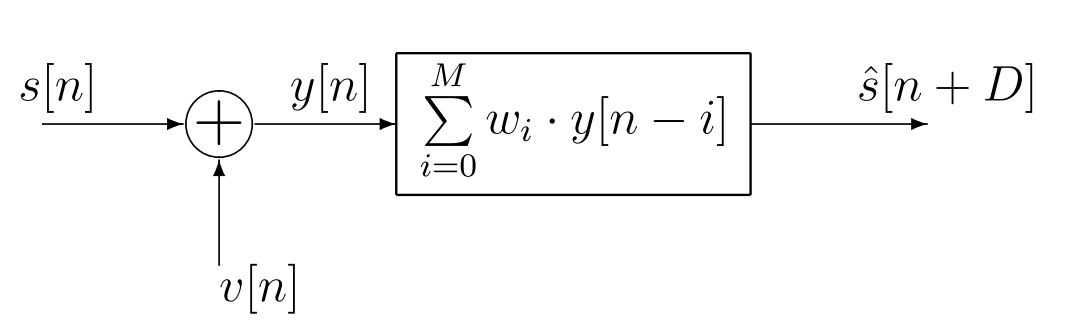
\includegraphics[width=\textwidth]{../fig/wiener_filter}
\end{minipage}
\begin{minipage}{.41\textwidth}
	\begin{itemize}[itemsep=1pt,topsep=3pt]
		\item $s[n]$: Ursprüngliches Signal
		\item $v[n]$: Störsignal (Rauschen)
		\item $\hat{s}[n+D]$: Schätzung von $s[n]$
	\end{itemize}	
\end{minipage}
~\\
Zurückgewonnenes Signal $\hat{s}[n+D]$.
\begin{itemize}[itemsep=1pt,topsep=3pt]
	\item \textit{Smoothing:} Bei $D<0$ ist der Sinn Rauschen vom Signal zu
	eliminieren und eine Verzögerung von $-D$ in Kauf zu nehmen. Für jedes Sample
	erzeugt der Filter eine Schätzung auf der Basis von $M+1$ Sampels von $y[n]$.
	\item \textit{Filtering:} Bei $D=0$ ist die Absicht das Signal $s[n]$ zu regenerieren.
	Es werden keine Verzögerungen erzeugt, da die Abschätzung aufgrund des 
	aktuellen und vergangenen Werten gemacht wird.
	\item \textit{Prediction:} Bei $D>0$ soll das Signal vorhergesagt werden.
\end{itemize} 
~\\
Filterausgang:
\[ \hat{s}[n+D] = \sum_{i=0}^{M}w_i\cdot y[n-i] \]
Schätz-Fehler:
\[ \hat{s}[n+D] - s[n+D] \]
Um die optimalen Parameter $w_i$ zu finden muss der Gradient auf Null gesetzt 
werden:
\[ \sum_{i=0}^{M}\tilde{w}_i \cdot \gamma_{yy}[m-i] = \gamma_{sy}[m+D], \qquad
	m=0,1,...,M \]
mit der Autokorrelation des Filter-Eingangs, rechts der Fall für das obige Modell:
\[ \gamma_{yy} = E\{ y[n] \cdot y^*[n-m] \} \qquad \qquad \gamma_{yy}[m] = \gamma_{ss}[m] + \gamma_{vv}[m] \]
und der Kreuzkorrelation, rechts der Fall für das obige Modell:
\[ \gamma_{sy} = E \{ s[n] \cdot y^*[n-m] \} \qquad \qquad \gamma_{sy}[m] = \gamma_{ss}[m] \]
~\\
Wiener-Hopf Gleichung:
\[ \textbf{R}_{yy} = \begin{bmatrix}
	\gamma_{yy}[0]	& \gamma_{yy}[-1]	& \ldots	& \gamma_{yy}[-M]\\
	\gamma_{yy}[1]	& \gamma_{yy}[0]	& \ldots	& \gamma_{yy}[1-M]\\
	\vdots			& \vdots			&			& \vdots\\
	\gamma_{yy}[M]	& \gamma_{yy}[M-1]	& \ldots	& \gamma_{yy}[0]
\end{bmatrix} \qquad \qquad
 \textbf{r}_{sy} = \begin{bmatrix}
	\gamma_{sy}[D]\\
	\gamma_{sy}[D+1]\\
	\vdots\\
	\gamma_{sy}[D+M]
\end{bmatrix} \qquad \qquad
  \tilde{\textbf{w}} = \begin{bmatrix}
	\tilde{w}_0\\
	\tilde{w}_1\\
	\vdots\\
	\tilde{w}_M
\end{bmatrix} \]
Der Vektor mit den optimalen Filterkoeffizienten $\tilde{\textbf{w}}$ ist gegeben durch:
\[ \tilde{\textbf{w}} = \textbf{R}_{yy}^{-1} \cdot \textbf{r}_{sy} \]
Anmerkung: Die Invertierung der Matrix $R_{yy}$ kann sich für hohe Ordnung $M$ als 
problematisch erweisen. Mittels \emph{Toeplitz}-Matrix lassen sich die Werte von 
$\tilde{w}$ ohne die Invertierung berechnen. 
%===============================================================================
\section{Kalman-Filter}
Jede zusätzliche Beobachtung wird für die Verbesserung der Filtercharakteristik verwendet, 
ohne dass die Ordnung limitierend wirkt. Basiert auf der Zustandsraumbeschreibung und 
eignet sich damit für dynamische Systeme.
\begin{center}
	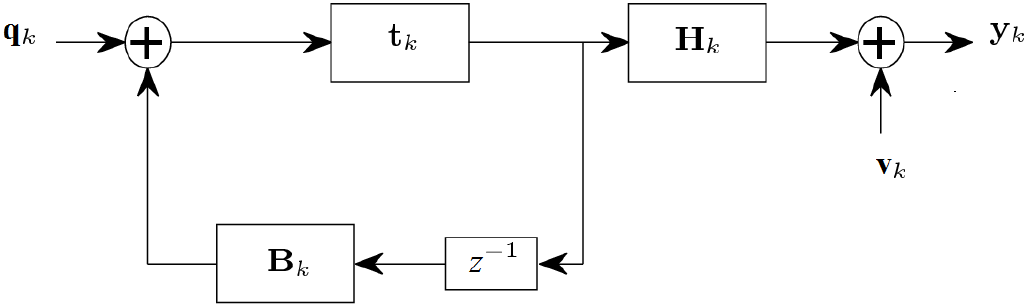
\includegraphics[width=0.6\textwidth]{../fig/kalmann_modell}
\end{center}
Von aussen sichtbar sind die Messwerte $\textbf{y}_1, \textbf{y}_2,...$. Für die $k$-te 
Beobachtung gilt:
\[ \textbf{y}_k = \textbf{H}_k \cdot \textbf{t}_k + \textbf{v}_k \]
Wobei $\textbf{H}_k$ die \emph{Messmatrix} und $\textbf{v}_k$ den Messfehler abbildet. \\\\
Für die internen Zustandsvariablen zum Zeitpunkt $k$ gilt:
\[ \textbf{t}_k = \textbf{B}_k \cdot \textbf{t}_{k-1} + \textbf{q}_k \]
Wobei $\textbf{B}_k$ die \emph{Zustandsübergangsmatrix} und $\textbf{q}_k$ den zufälliger 
Vektor ist. \\\\
\textbf{Übersicht über die Filter-Bestandteile:}
\begin{flushleft}
	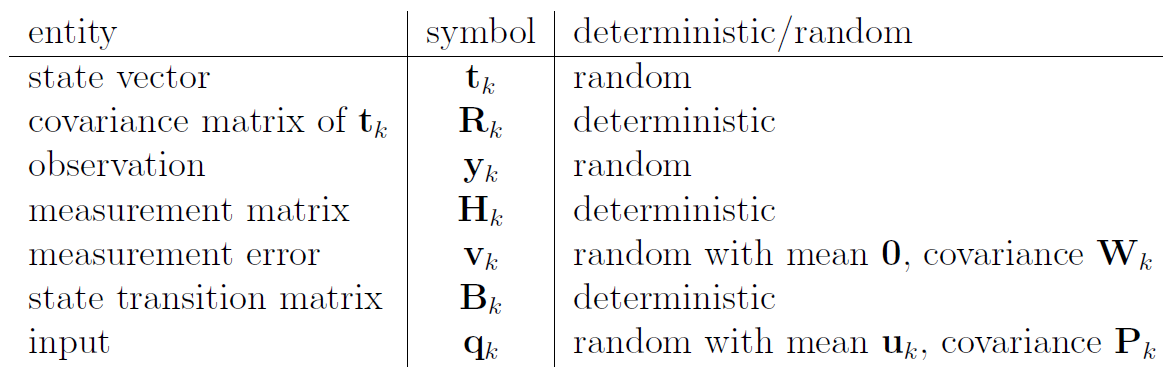
\includegraphics[width=0.625\textwidth]{../fig/kalmann_bestandteile}
\end{flushleft}
\textbf{Vergleich zum Wiener-Filter:\\}
Beide Filter sind optimale lineare Filter bezüglich dem mean-squared error. 
Der Wiener-Filter hat eine endliche Ordnung $M$, der Kalman-Filter hingegen
ist rekursiv aufgebaut und hat keine endliche Ordnung. Der Kalman-Filter 
eignet sich im Gegensatz zum Wiener-Filter für dynamische Systeme statt
nur für stationäre Systeme.